\documentclass[letterpaper,12pt]{amsart}

\usepackage{ucs}
\usepackage[utf8x]{inputenc}
\usepackage{amsmath}
%\usepackage{amsfonts}
%\usepackage{amssymb}
\usepackage[margin=1in]{geometry}
\usepackage{graphicx}
\usepackage[bitstream-charter]{mathdesign}
\usepackage[T1]{fontenc}

\newcommand{\len}[1]{\lVert #1\rVert}
\newcommand{\abs}[1]{\left\lvert #1\right\rvert}
\newcommand{\R}{\mathbb{R}}
\title{Math 1410 Assignment \#1 Solutions\\University of Lethbridge, Fall 2016}
\author{Sean Fitzpatrick}
\begin{document}
 \maketitle

\begin{enumerate}
\item Show that for \textbf{any} complex numbers $z$ and $w$, with $w\neq 0$, the complex modulus satisfies
\[
 \left\lvert\frac{z}{w}\right\rvert = \frac{\abs{z}}{\abs{w}}.
\]

\medskip

\textbf{Solution:} from the textbook, we have the proof that the complex modulus satisfies $\abs{zw}=\abs{z}\abs{w}$. Following the suggestion in the text, we have
\[
 \abs{\frac{z}{w}} = \abs{z\left(\frac{1}{w}\right)} = \abs{z}\abs{\frac{1}{w}},
\]
where in the last equality we've used the product rule for the modulus given above. Thus, it suffices to show that $\left\lvert\dfrac{1}{w}\right\rvert = \dfrac{1}{\abs{w}}$ for any nonzero complex number $w$, since we would then have
\[
 \abs{\frac{z}{w}} = \abs{z}\abs{\frac{1}{w}} = \abs{z}\left(\frac{1}{\abs{w}}\right) = \frac{\abs{z}}{\abs{w}}.
\]
To show this, we let $w=u+iv$, where $u$ and $v$ can be any real numbers (as long as they're not both zero). We then have
\[
 \frac{1}{w} = \frac{1}{u+iv} = \frac{1}{u+iv}\frac{u-iv}{u-iv} = \frac{u-iv}{u^2+v^2} = \left(\frac{u}{u^2+v^2}\right)+i\left(\frac{-v}{u^2+v^2}\right).
\]
The modulus of $\dfrac{1}{w}$ is therefore
\begin{align*}
 \abs{\frac{1}{w}} & = \sqrt{\left(\frac{u}{u^2+v^2}\right)^2+\left(\frac{-v}{u^2+v^2}\right)^2}\\
 & = \sqrt{\frac{u^2}{(u^2+v^2)^2}+\frac{v^2}{(u^2+v^2)^2}} = \sqrt{\frac{u^2+v^2}{(u^2+v^2)^2}}\\
 & = \sqrt{\frac{1}{u^2+v^2}} = \frac{1}{\sqrt{u^2+v^2}} = \frac{1}{\abs{w}},
\end{align*}
as required.

\item Compute the following complex roots, and plot them in the complex plane. \\(See Example 14 on page 47 of the text for guidance.)

\medskip

\begin{enumerate}
 \item Find the three cube roots of $z=-125$.

\bigskip

We first convert $z$ to polar form: we have $z=-125 = 125(-1) = 125e^{i\pi} = 125e^{i(\pi+k(2\pi))}$, since we can add any multiple of $2\pi$ to the argument without changing the value of $z$. If $w$ is a cube root of $z$, then we must have $w^3=z$. Writing $w=re^{i\theta}$ in polar form, we have
\[
 w^3 = r^3e^{i(3\theta)} = 125e^{i(\pi+k(2\pi))}, \text{ for } k=0,1,2,\ldots
\]
Comparing these two numbers in polar form, we must have $r^3=125$, giving us $r=5$, and $3\theta = \pi+(2k)\pi$, for some integer value of $k$. Solving for $\theta$, we have
\[
 \theta = \frac{\pi}{3} + \left(\frac{2k\pi}{3}\right).
\]
We obtain three distinct cube roots of $z$ by taking $k=0$, 1, and 2. (Choosing $k=3$ gives us $\frac{\pi}{3}+2\pi$, resulting in the same complex number as $k=0$, and all other values of $k$ similarly repeat the existing values.) Our solutions are thus
\begin{align*}
 w_0 & = 5e^{i(\pi/3)} = 5(\cos(\pi/3)+i\sin(\pi/3)) = 5\left(\frac{1}{2}+i\frac{\sqrt{3}}{2}\right) = \frac{5}{2}+i\frac{5\sqrt{3}}{2}\\
 w_1 & = 5e^{i(\pi/3+2\pi/3)} = 5e^{i\pi} = -5.\\
 w_2 & = 5e^{i(\pi/3+4\pi/3)} = 5e^{i(5\pi/3)} = 5(\cos(5\pi/3)+i\sin(5\pi/3)) = \frac{5}{2}-i\frac{5\sqrt{3}}{2}.
\end{align*}
The three roots are plotted as shown:
\begin{center}
 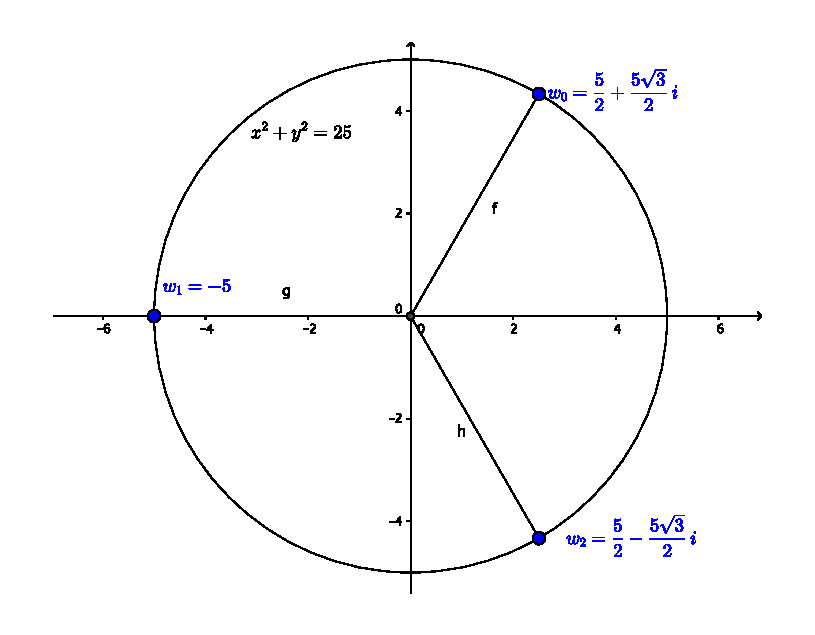
\includegraphics[width=4in]{A1_2a_sol}
\end{center}



 \item Find the six 6th roots of $z=64$.

Again, we first write $z=64=64e^{i(2\pi k)}$, where $k$ can be any integer. If $w=re^{i\theta}$ is a sixth root of $z$, then we must have
\[
 w^6 = r^6e^{i(6\theta)} = 64e^{i(2\pi k)}, \text{ for } k=0, 1, 2, \ldots
\]
Comparing our two complex numbers, we must have $r^6=64$, so $r=2$, and $6\theta = 2\pi k$, giving us
\[
 \theta = k\left(\frac{2\pi}{6}\right)=k\left(\frac{\pi}{3}\right), \text{ where } k=0,1,2,3,4,5.
\]
Again, we do not need to consider values of $k\geq 6$, since $6(\pi/3)=2\pi$ corresponds to the same point as $k=0$, and all other values repeat similarly. The six cube roots are thus
\begin{align*}
 w_0 & = 2e^{i(0)} = 2,\\
 w_1 & = 2e^{i(\pi/3)} = 2\left(\frac{1}{2}+\frac{\sqrt{3}}{2}i\right) = 1+i\sqrt{3},
 w_2 & = 2e^{i(2\pi/3)} = -1+i\sqrt{3},\\
 w_3 & = 2e^{i(3\pi/3)} = 2e^{i\pi} = -2,\\
 w_4 & = 2e^{i(4\pi/3)} = -1-i\sqrt{3},\\
 w_5 & = 2e^{i(5\pi/3)} = 1-i\sqrt{3}.
\end{align*}
The six roots can all be plotted on the circle $x^2+y^2=4$ as follows:
\begin{center}
 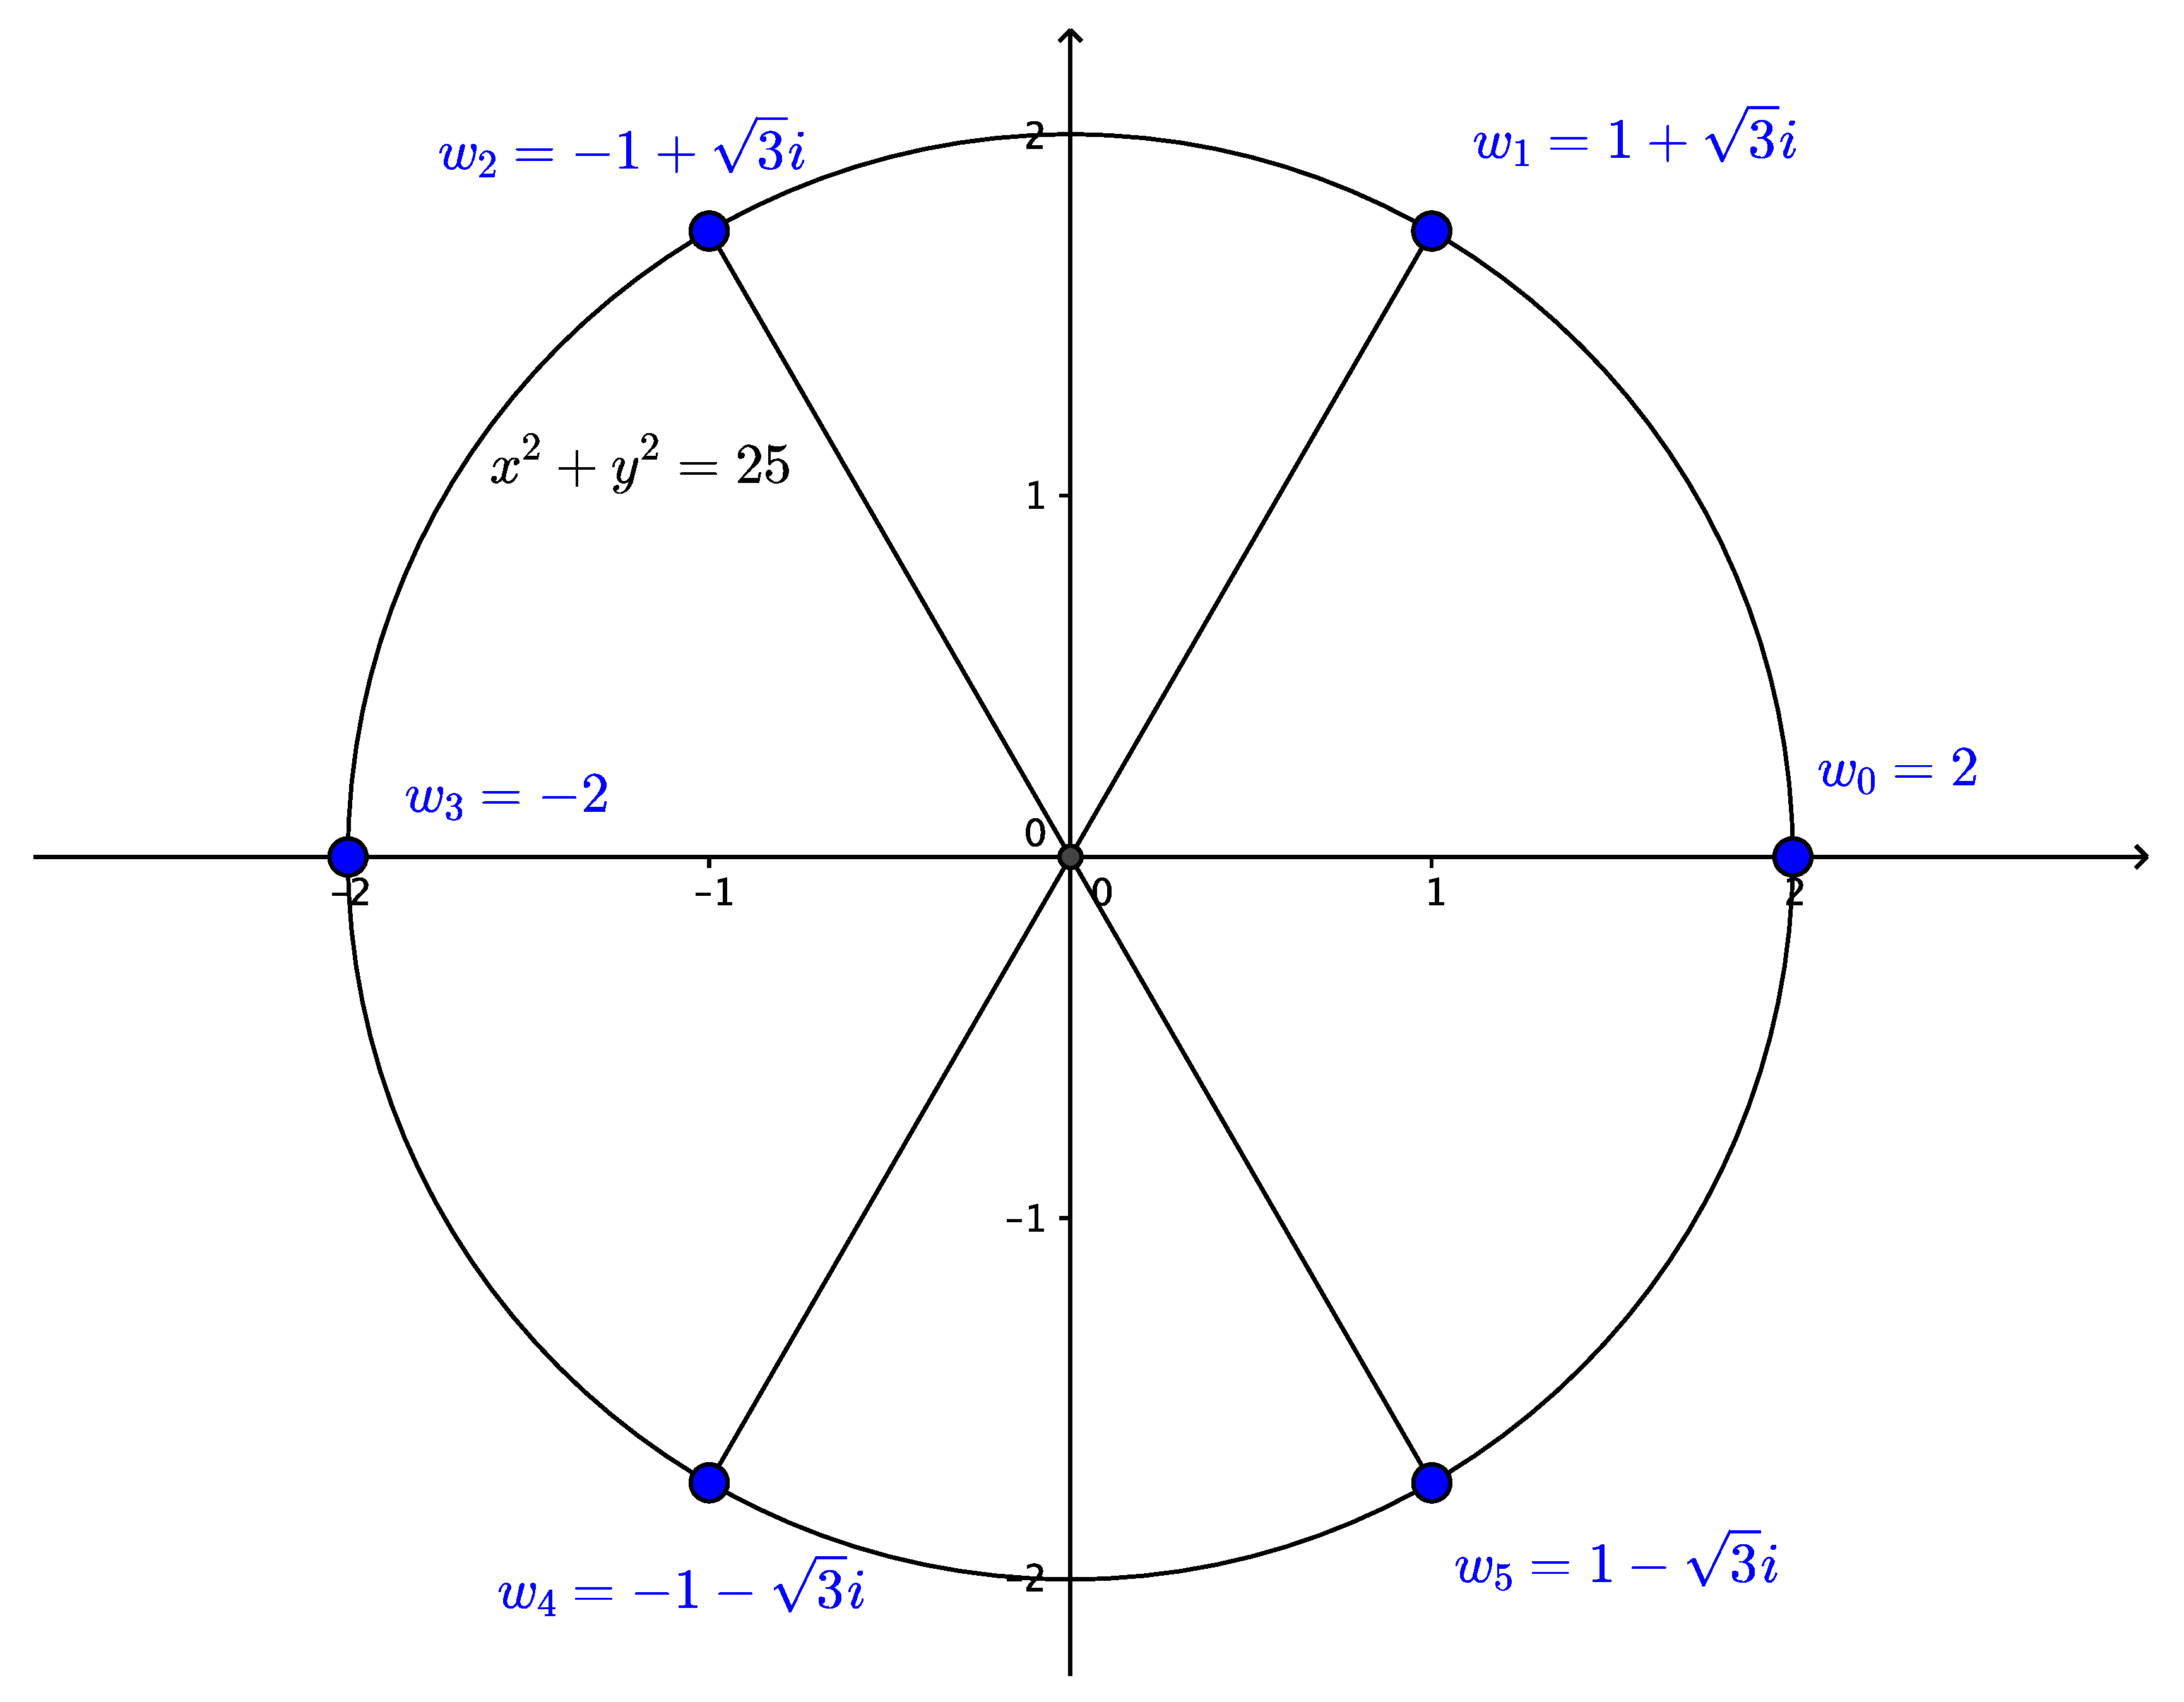
\includegraphics[width=4in]{A1_2b_sol}
\end{center}


\end{enumerate}

\medskip



\bigskip

\item Let $\vec{v}$ and $\vec{w}$ be vectors in $\R^3$. In each case, either explain why the statement is true (in general), or give an example showing that it is false:

\medskip

\begin{enumerate}
 \item If $\len{\vec{v}-\vec{w}}=0$, then $\vec{v}=\vec{w}$.

\medskip

This is true. We know that the only vector with zero length is the zero vector, so if $\len{\vec{v}-\vec{w}}=0$, then we must have $\vec{v}-\vec{w} = \vec{0}$, and therefore $\vec{v}=\vec{w}$.

 \item If $\vec{v}=-\vec{v}$, then $\vec{v}=\vec{0}$.

\medskip

This is true. Supposing that $\vec{v}=-\vec{v}$, we can add $\vec{v}$ to both sides, giving us $\vec{v}+\vec{v} = 2\vec{v} = \vec{0}$. But if $2\vec{v}=\vec{0}$, we can multiply both sides of this equation by $\frac{1}{2}$, giving us
\[
 \vec{0} = \frac{1}{2}\vec{0} = \frac{1}{2}(2\vec{v}) = \left(\frac{1}{2}(2)\right)\vec{v} = 1\vec{v} = \vec{v}.
\]

 \item If $\len{\vec{v}}=\len{\vec{w}}$, then $\vec{v}=\vec{w}$.

\medskip

This is false. There are in fact infinitely many vectors of a given length. To provide just one example, if $\vec{v}=\langle 1,0\rangle$ $\vec{w} = \langle 0,1\rangle$, then $\vec{v}\neq \vec{w}$, but $\len{\vec{v}}=\len{\vec{w}}$.

 \item If $\len{\vec{v}}=\len{\vec{w}}$, then $\vec{v}=\pm\vec{w}$.

\medskip

This is also false, and the same example given for the previous problem applies.

 \item $\len{\vec{v}+\vec{w}} = \len{\vec{v}}+\len{\vec{w}}$.

This is false. For example, let $\vec{v}=\langle 1,0\rangle$ and let $\vec{w} = \langle 0,1\rangle$. Then $\vec{v}+\vec{w} = \langle 1,1\rangle$, so
\[
 \len{\vec{v}+\vec{w}} = \sqrt{1^2+1^2}=\sqrt{2},
\]
but $\len{\vec{v}}+\len{\vec{w}} = 1+1=2\neq \sqrt{2}$.
\end{enumerate}

\bigskip

\item Consider the triangle in $\R^3$ with vertices (corners) at the points 
\[
P=(2,0,-3),\, Q=(5,-2,1),\, \text{ and } R=(7,5,3). 
\]
 Show that this is a right-angled triangle

\medskip

\begin{enumerate}
 \item Using dot products.

\medskip

Consider the vectors $\overrightarrow{QP} = \langle -3,2,-4\rangle$ and $\overrightarrow{QR} = \langle 2, 7, 2\rangle$. We have
\[
 \overrightarrow{QP}\boldsymbol{\cdot}\overrightarrow{QR} = (-3)(2)+2(7)-4(2) = -6+14-8=0.
\]
Since these two vectors, which form two sides of the given triangle, are orthogonal, the given triangle must be a right-angled triangle.

(Note that there are three possible corners with three possible angles. To solve this, you just need to work through the three different possible pairs of vectors until you find the one that's orthogonal. There's no need to write out the ones that didn't work.)

 \item Using the Pythagorean Theorem.

\medskip

We compute the lengths of the three sides of the triangle:
\begin{align*}
 d(P,Q) & = \len{\overrightarrow{PQ}} = \sqrt{3^2+(-2)^2+4^2} = \sqrt{29}\\
 d(Q,R) & = \len{\overrightarrow{QR}} = \sqrt{2^2+7^2+2^2} = \sqrt{57}\\
 d(P,R) & = \len{\overrightarrow{PR}} = \sqrt{5^2+5^2+6^2} = \sqrt{86},
\end{align*}
and
\[
 d(P,Q)^2+d(Q,R)^2 = \sqrt{29}^2+\sqrt{57}^2 = 29+57=86=\sqrt{86}^2 = d(P,R)^2,
\]
so the three side lengths satisfy the Pythagorean Theorem.

\end{enumerate}
\end{enumerate}

\end{document}
 
